\section{Formulación como problema de control}
\begin{frame}
    \frametitle{Problema de Control}
    \begin{problem}[OCP para SHE de dos niveles]\label{OCP1}
        \begin{itemize}
            \item Consideramos dos conjuntos de números impares $\mathcal{E}_a$ and $\mathcal{E}_b$ con cardinalidades $|\mathcal{E}_a| = N_a$ y  $|\mathcal{E}_b| = N_b$.
            \item Consideramos los vectores objetivos $\bm{a}_T  \in \mathbb{R}^{N_a}$ y $\bm{b}_T  \in \mathbb{R}^{N_b}$.
            \item Buscamos la función  $f(\tau ) \ | \ \tau \in (0,\pi)$ que minimiza el siguiente funcional de coste:

        \end{itemize}
            \begin{gather}
            J[f(\tau)] =  \| \bm{a}_T - \bm{\alpha}(T)\|^2 + \| \bm{b}_T - \bm{\beta}(T)\|^2 
            + \epsilon \int_0^{\pi} \mathcal{L}(f) d\tau  
        \end{gather}
    \end{problem}
\end{frame}

\begin{frame}
    \frametitle{}
    \begin{problem}[OCP para SHE de dos niveles]
    De esta forma podemos escribir el siguiente problema de control óptimo:
    \begin{gather}
        \min_{|f(\tau) |<1} J[f(\tau)] \\
        \notag \text{suject to: } \\
        \notag \forall i \in \mathcal{E}_a\ \ 
        \begin{cases}
            \dot{\alpha}_i(\tau) = (2/\pi) \cos(i\tau) f(\tau) & \tau \in [0,\pi]\label{dyn}\\
            \alpha_i(0) = 0
        \end{cases} \\
        \notag \forall j \in \mathcal{E}_b\ \ 
        \begin{cases}
            \dot{\beta}_j(\tau) = (2/\pi) \sin(j\tau) f(\tau) & \tau \in [0,\pi]\label{dyn}\\
            \beta_j(0) = 0
        \end{cases} \\
    \end{gather}
    \end{problem}
\end{frame}



\begin{frame}
    \frametitle{Condiciones de optimalidad}

    Es necesario construir la función Hamiltoniana:
    \begin{gather}\label{hamil}
        H(f,\bm{p}^\alpha,\bm{p}^\beta,\tau) = \epsilon \mathcal{L}(f) + 
        G(\bm{p}^\alpha,\bm{p}^\beta,\tau) f
    \end{gather}
    Donde  hemos llamado $G(\bm{p}^\alpha,\bm{p}^\beta,\tau)$ a:
    \begin{gather}
        G(\bm{p}^\alpha,\bm{p}^\beta,\tau) = \frac{2}{\pi} \Bigg[ 
            \sum_{i \in \mathcal{E}_a} p^\alpha_i \cos(i\tau)+ 
            \sum_{j \in \mathcal{E}_b} p^\beta_j \sin(j\tau) 
        \Bigg]
    \end{gather}
    Y donde $\bm{p}^\alpha$ y $\bm{p}^\beta$ son los co-estados del sistema.
\end{frame}


\begin{frame}
    \frametitle{Principio de mínimo de Pontryagin}
    Cuando evaluamos el Hamiltoniano en los co-estados óptimos $\bm{p}_*^\alpha$ y $\bm{p}_*^\beta$ podemos encontrar la forma del control minimizando el Hamiltoniano.
    \begin{gather}\label{minH}
        H(\tau,\bm{p}_*^\alpha,\bm{p}^\beta_*,f_*) \leq
        H(\tau,\bm{p}_*^\alpha,\bm{p}^\beta_*,f)
    \end{gather}
    Entonces anilizaremos el problema 
    \begin{gather}
        \min_{|f|<1} H_*(f)
    \end{gather}
    Donde hemos llamado $H_*(f)$ a $H(\tau,\bm{p}_*^\alpha,\bm{p}^\beta_*,f)$
\end{frame}


\begin{frame}
    \frametitle{Condiciones necesarias de optimalidad}
    Entonces las condiciones necesarias de optimialidad para este problema se puede escribir como:
    \begin{gather}\label{hamil}
        H_*(f) = \epsilon \mathcal{L}(f) + 
        G(\bm{p}^\alpha_*,\bm{p}^\beta_*,\tau) f \\
        \frac{dH_*(f)}{df} = 0 \\
        \frac{dH_*^2(f)}{df^2} \geq 0 
    \end{gather}

\end{frame}

\begin{frame}
    \frametitle{Condiciones necesarias de optimalidad}
    Entonces las condiciones necesarias de optimialidad para este problema se puede escribir como:
    \begin{align}\label{hamil}
        H_*(f) = & \epsilon \mathcal{L}(f) + 
        G(\bm{p}^\alpha_*,\bm{p}^\beta_*,\tau) f \\
        \frac{dH_*(f)}{df} =  & \epsilon\frac{d\mathcal{L}}{df} + G(\bm{p}^\alpha_*,\bm{p}^\beta_*,\tau) = 0\\
        \frac{dH_*^2(f)}{df^2} = &  \epsilon \frac{d\mathcal{L}^2}{df^2}\geq 0 
    \end{align}

\end{frame}

\begin{frame}
    \frametitle{}
    \begin{figure}
        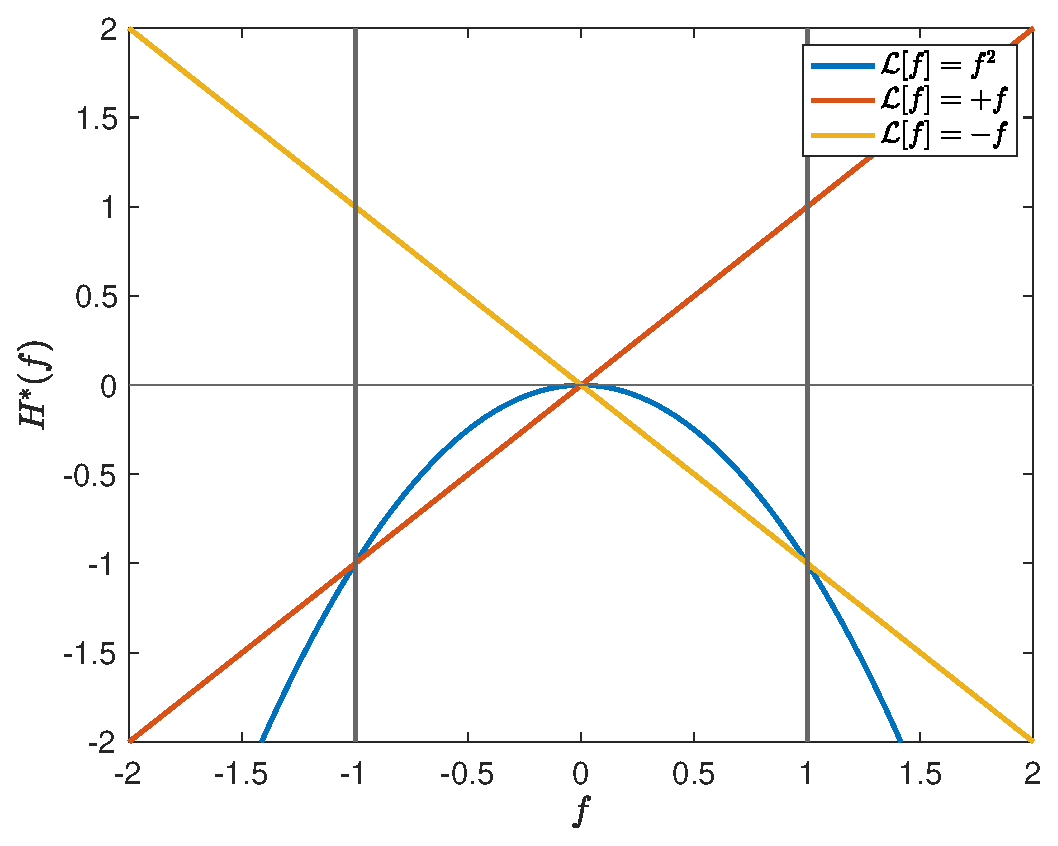
\includegraphics[scale=0.45]{imgs/bang-bang.eps}
    \end{figure}
\end{frame}
